\chapter{Related work} \label{cap:literatura}
  
This chapter describes the main related projects found in the literature referenced in this work. The first section mentions the first literary reference found in the execution of this work that performs comparisons of demand forecasting methods. The second section mentions research related to the theme of this work, the prediction of demand in university refectory, containing studies related to a part of the methods performed in this work which are the models of MLP neural networks and the differential of this work in relation to others is the inclusion of modern recurrent neural networks called GRU based on the topic \ref{sec:GRU}. The last section mentions the largest volume of references found during general demand prediction surveys, and which did not correspond to the topic of this monograph.

    \section{Comparison work of demand forecasting methods.}
       \citeonline{Junior2007} develops a comparison between stochastic methods (Exponential Smoothing Method, Box-Jenkins models) and machine learning models (Neural Networks), illustrated in Figures \ref{fig: metodosPrevisaoDemanda}, which are used to forecast the demand for cosmetic products distributed in time series. Among the Neural Networks, we find networks such as \textit{feedforward} with the \textit{backpropagation} training algorithm that was the main focus of the R.U. prediction project at the Federal University of Viçosa and the State University of Paulista Júlio de Mesquita Filho that also underpinned part of the development of this prediction work at ICT Unifesp. In this work of the author, we also analyze several predictive performance measures and make a final comparative analysis of these measures between the cited methods.
    
    \section{Forecast demand in university refectory}
        In the statistical study by \citeonline{Landim2016}, In the study by Dougkf, was analyzed the correlation between temperature and meal consumption on sales days of the university restaurant of the ICT-Unifesp campus, where the data contained only a small sample of sales of the second half of 2016. Because of low volume of occurrences, the data was submitted to re-sampling via bootstrap. According to the sample graphs, it was identified that the correlation shown in the graphs of the first half of the semester and the total semester formed bimodal distributions. However, in the second half of the semester it formed a unimodal distribution. The conclusion was that other variables and other analysis models should be used for this demand forecasting.
        
        \citeonline{Lopes2008} makes the same study of this scenario of ICT-Unifesp applied at the Federal University of Viçosa (UFV). In this study, the data used were only the university refectory's sales history, and no environment variables were collected such as temperature, precipitation, number of students enrolled, etc. The algorithm used was \textit{Traincgp (Conjugate gradient backpropagation with Polak-Ribiere updates)} in software Matlab. This algorithm does not involve the calculation of second derivatives of variables and converges at least the quadratic function into a finite number of iterations as quoted by the author. For each node of the neural net, the day of the week (such as Monday, Tuesday, Wednesday, Thursday and Friday) and each layer of this net using the previous 5 days for each node (the previous 5 seconds, 5 Tuesdays and so on) were then considered and, finally, a model was obtained by the net that presented a maximum error of 3. The neural net applied in this work is represented in Figure \ref{fig:mlp-lopes}.
        
        \begin{figure}[h]
        \center{
        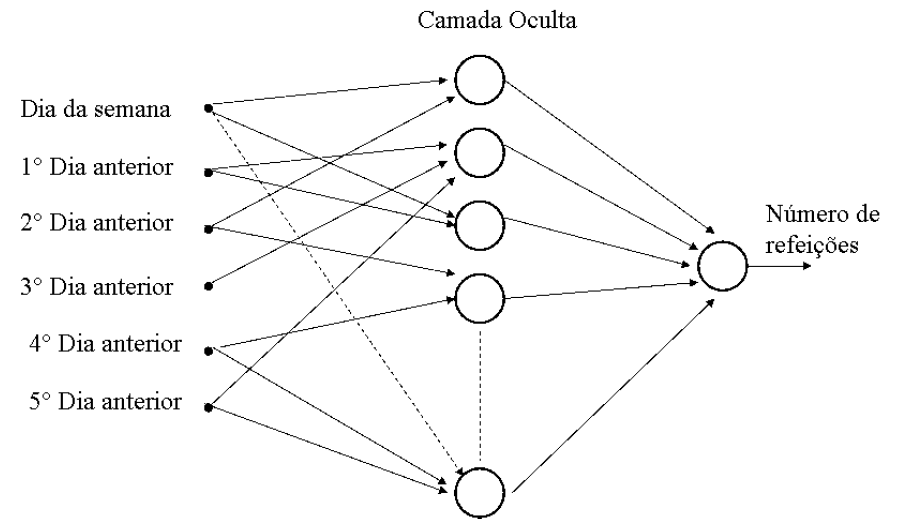
\includegraphics[width=\textwidth]
        {./Figs/15-rna-lopes.png}
        \caption{Multiple Layer Perceptron Neural Network.}\caption*{  Fonte:\cite{Lopes2008}.}\label{fig:mlp-lopes}}
        \end{figure}
        
        \citeonline{Rocha2011} also performs the demand study at the Universidade Estadual Paulista Júlio de Mesquita Filho (UNESP) university restaurant, again with the methods of artificial neural networks with backpropagation and using only as data source (the numerical history of sales made), and other intermediate variables obtained from this, as means of subset of observations (Monday averages). The only environment variable collected was the number of holidays close to the sales observation. In the study of the total number of days analyzed, it can be seen that in 73\% (187 days), the simple average method provided a greater error in relation to RNA, which in turn caused a greater error in the remaining 23\% (69 days). In the case of less waste, it can be observed that RNA presents errors greater than 50 meals in 13 days, while the simple average method presents errors greater than 50 meals in 58 days, concluding then that the RNA method was much more efficient than the simple average calculation used by the administration of the university restaurant. The Figure \ref{fig:rnaRocha} shows a Neural Network scheme applied in this research. 
        \begin{figure}[h]
        \center{
        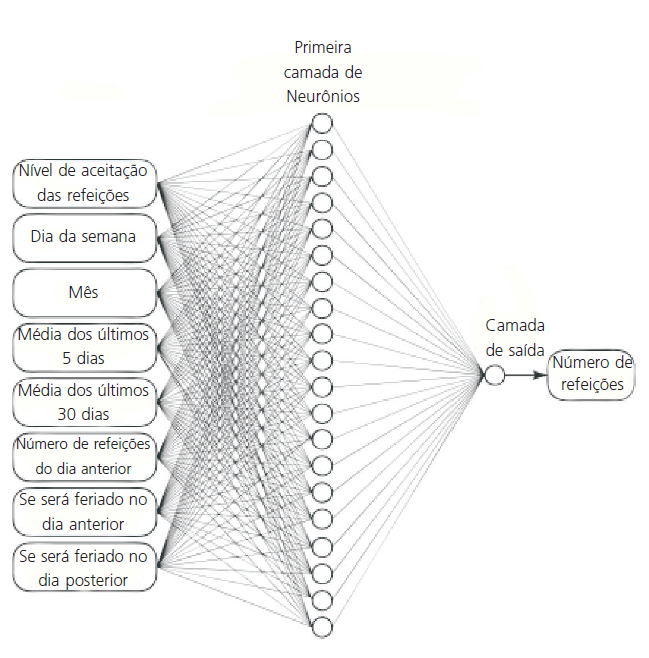
\includegraphics[width=0.8\textwidth]
        {./Figs/16-rna-rocha.png}
        \caption{Multiple Layer Perceptron Neural Network}\caption*{ Fonte: \cite{Rocha2011}} \label{fig:rnaRocha}}
        \end{figure}
        
        Both the model presented in \cite{Rocha2011} as in \cite{Lopes2008} have a single hidden layer.
      
    \section{Demand forecasting in other scenarios.}
        \citeonline{RUAS2012}makes an analysis of demand forecasting for electricity in the state of Paraná, between the years 2004 and 2006, using Artificial Neural Networks and support vector machines. Although it is not the same example of the ICT-Unifesp university refectory scenario, we have the distribution of the consumption data collected as a time series. In this research for forecasting electricity demand a partially recurring Elman network was used, which allows the prediction of a step forward. To be possible to make the forecast for several points ahead it is necessary to use the values already predicted, that means the output of the network, as inputs to it.
        
        \citeonline{Almeida2013} analyzes a similar scenario of electric power demand, but using demand forecasting techniques with Artificial Multilayer Perceptron type Neural Network combined with fuzzy logic that allows placing temperature variables (among others) in a set of rules that impact the problem.
        
        \citeonline{Silva2010} also applies Neural Network techniques to predict electric power demand, with the study of climatic variables, but through a SOM MAP model - (Self-Organizing Map) which is a type of neural network developed for pattern recognition. Despite being an unsupervised model, the model is ideal for organizing the main impacting and disposable variables in the forecast. The sound map used by the author presents the data associated to his neurons so that similar patterns are found in contiguous neurons, having a topological organization. That way it is possible to extract abstract relations between the variables of the data vector through their position in the component maps, which through a color scale show the amount of a specific variable in each neuron of the map.